% Prof. Dr. Ausberto S. Castro Vera
% UENF - CCT - LCMAT - Curso de Ciência da Computação
% Campos, RJ,  2023
% Disciplina: Paradigmas de Linguagens de Programação
% Aluno: Mariana Cossetti Dalfior

%%%*****************************************************************************************%%%
\chapter{Introdu\c{c}\~{a}o}
%%%*****************************************************************************************%%%

De acordo com \cite{Tulchak2016}, a linguagem de programa\c{c}\~{a}o Python foi idealizada inicialmente por Guido van Rossum no in\'{\i}cio dos anos 1990. Ela \'{e} sucessora da linguagem ABC e possui seu nome inspirado em um grupo de com\'{e}dia chamado Monty Python. Python \'{e} uma linguagem interpretada, o que significa que ela utiliza um int\'{e}rprete que permite ler o c\'{o}digo linha por linha sem a necessidade de compilar o c\'{o}digo completo de uma vez. \'{E} considerada uma linguagem de alto n\'{\i}vel, assim como PHP, Java, Fortran e C, por\'{e}m, possui como diferencial a sua sintaxe clara e concisa, a rapidez de processamento e uma maior regularidade que as outras linguagens de alto n\'{\i}vel, tornando-se mais f\'{a}cil de ler e aprender.

Al\'{e}m de ser uma linguagem de programa\c{c}\~{a}o orientada a objetos, o que significa que os programas s\~{a}o constru\'{\i}dos em torno de objetos que podem ser determinados e manipulados pelo programador, Python tamb\'{e}m \'{e} uma linguagem de multiplataforma. Isso significa que ela pode ser executada em diversos sistemas operacionais, como Windows, MacOS e Linux, possibilitando que os desenvolvedores elaborem programas capazes de serem executados em diferentes plataformas sem que ocorram grandes modifica\c{c}\~{o}es no c\'{o}digo.

Python apresenta uma ampla diversidade de bibliotecas, dentre elas destacam-se Pandas, Numpy, Matplotlib, Pillow, Scikit-learn e TensorFlow. Devido \`{a} facilidade e rapidez proporcionada pela grande variedade de bibliotecas e m\'{o}dulos, essa linguagem \'{e} amplamente empregada em Data Science, IA (Intelig\^{e}ncia Artificial), Machine Learning (Aprendizado de M\'{a}quina), automa\c{c}\~{a}o, desenvolvimento web e outros campos.


%%%=========================================================================================%%%
   \section{Aspectos hist\'{o}ricos da linguagem Python}
%%%=========================================================================================%%%

A hist\'{o}ria da linguagem de programa\c{c}\~{a}o Python vem sendo desenvolvida desde a sua cria\c{c}\~{a}o no in\'{\i}cio da d\'{e}cada de 1990 at\'{e} os dias atuais, a qual foi se tornando cada vez mais popular.

Relata-se a seguir alguns aspectos hist\'{o}ricos dessa linguagem. As informações exibidas logo a seguir foram baseadas em  (\url{https://docs.python.org/3/whatsnew/index.html}), \cite{Rossum2010, Silva2019, Montoro2012} :

\begin{itemize} [itemsep=5pt, parsep=5pt]

\item O principal autor da linguagem Python foi o Guido van Rossum.

\item Divergente do que acreditam, Python n\~{a}o obteve esse nome devido a esp\'{e}cie de serpente P\'{\i}ton. Ele foi nomeado assim em homenagem a um seriado de com\'{e}dia. \textit{Monty Python's Flying Circus} de que Guido van Rossum era f\~{a}.

\item Python conquistou uma certa popularidade em \'{a}reas espec\'{\i}ficas, como processamento de texto e  computa\c{c}\~{a}o cient\'{\i}fica, durante a d\'{e}cada de 1990.

\item No ano 1991, foi lan\c{c}ada a primeira vers\~{a}o p\'{u}blica do Python o 0.9.0. Nela foi inclu\'{\i}da suporte para a manipula\c{c}\~{a}o de estruturas de controle de fluxo, strings e fun\c{c}\~{o}es. Al\'{e}m da inclus\~{a}o de algumas caracter\'{\i}sticas de programa\c{c}\~{a}o funcional.

\item No ano 1994, van Rossum lan\c{c}ou a vers\~{a}o 1.0 do Python, que adicionou novos recursos e melhorias \`{a} linguagem, como suporte para orienta\c{c}\~{a}o a objetos e para m\'{o}dulos e pacotes.

\item Guido lan\c{c}ou a vers\~{a}o 1.2 do Python antes de desligar-se do seu emprego na CWI

\item Em 1995, Guido lan\c{c}ou novas vers\~{o}es do Pyhton enquanto trabalhava em uma nova empresa CNRI (Corporation for National Research Initiatives) em Reston, nos Estados Unidos. Uma delas foi a vers\~{a}o 1.4, a qual foi implementada o suporte nativo a n\'{u}meros complexos e par\^{a}metros nomeados.

\item Python 1.6 foi a \'{u}ltima vers\~{a}o a ser lan\c{c}ada na CNRI, no ano de 2000.

\item Em 2000, tamb\'{e}m foi lan\c{c}ada a vers\~{a}o Python 2.0 na BeOpen, entretanto foi o \'{u}nico lan\c{c}amento nessa empresa. Implementando um sistema de coletor de lixo com capacidade de tratar ciclos de refer\^{e}ncias e tamb\'{e}m a list comprehension (Compreens\~{a}o de listas).

\item Python ganhou bastante popularidade do in\'{\i}cio de 2000, com o uso crescente de Python em Data Science e Machine Learning.

\item A vers\~{a}o Python 2.1 era semelhante as vers\~{o}es 1.6.1 e 2.0, a qual recebeu as mudan\c{c}as na especifica\c{c}\~{a}o que suporte escopo aninhado e foi lan\c{c}ada em 2001.

\item Tamb\'{e}m em 2001 a vers\~{a}o Python 2.2 lan\c{c}ada e possuiu uma grande novidade, em que houve a uni\~{a}o dos tipos Python - que eram escritos em C - e as classes - que j\'{a} eram escritas em Python - em uma s\'{o} hierarquia.

\item Em 2008 foi publicado Python 2.6, j\'{a} com a inten\c{c}\~{a}o de fazer a transi\c{c}\~{a}o dele para o Python 3.0. Uma nova maneira de formatar strings e bibliotecas para multiprocessamento foi inclu\'{\i}da na vers\~{a}o 2.6.

\item Tamb\'{e}m em 2008 foi lan\c{c}ada Python 3.0, que introduziu mudan\c{c}as na sintaxe e manipula\c{c}\~{a}o de strings. Tornando Python mais f\'{a}cil de aprender, por\'{e}m isso gerou algumas incompatibilidades com vers\~{o}es mais antigas.

\item No ano de 2010, foi criado um framework Django para facilitar o desenvolvimento de aplica\c{c}\~{o}es web na linguagem de programa\c{c}\~{a}o Python.

\item O PEP 484, foi aprovado em 2015, possibilitando adicionar tipos opcionais ao Python. Essa mudan\c{c}a foi projetada com o intuito de ajudar os desenvolvedores a escreverem um c\'{o}digo mais confi\'{a}vel e seguro. Nesse ano tamb\'{e}m foi lan\c{c}ada a vers\~{a}o Python 3.5.

\item Entre 2015 e 2023 foram lan\c{c}adas as vers\~{o}es desde a Python 3.6 at\'{e} Python 3.11. Nessas novas vers\~{o}es foram adicionadas melhorias no interpretador, na sintaxe, velocidade, biblioteca padr\~{a}o e etc. 

\end{itemize}

\begin{figure}[H]
\begin{center}
		\caption{Progress\~{a}o das vers\~{o}es do Python} \label{ling1}
		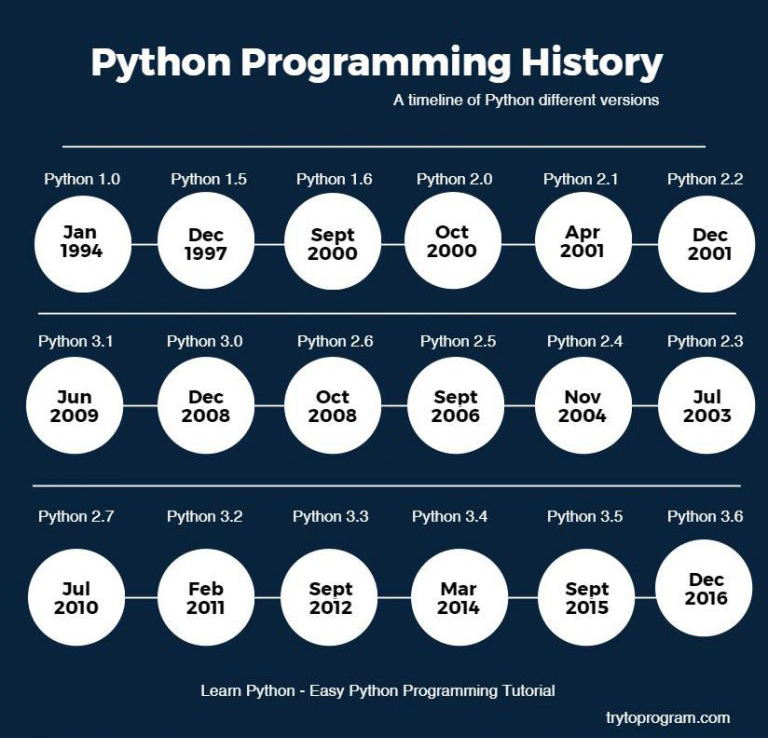
\includegraphics[width=12cm]{pythonhistory} \newline
		Fonte: \url{www.tryprogram.com}
\end{center}
\end{figure}

A seguir \'{e} poss\'{\i}vel observar algumas logotipos da linguagem Python que foram desenvolvidas com o passar dos anos:

\begin{figure}[H]
\begin{center}
	\caption{Logos da Linguagem Python}
	\label{ling2}
	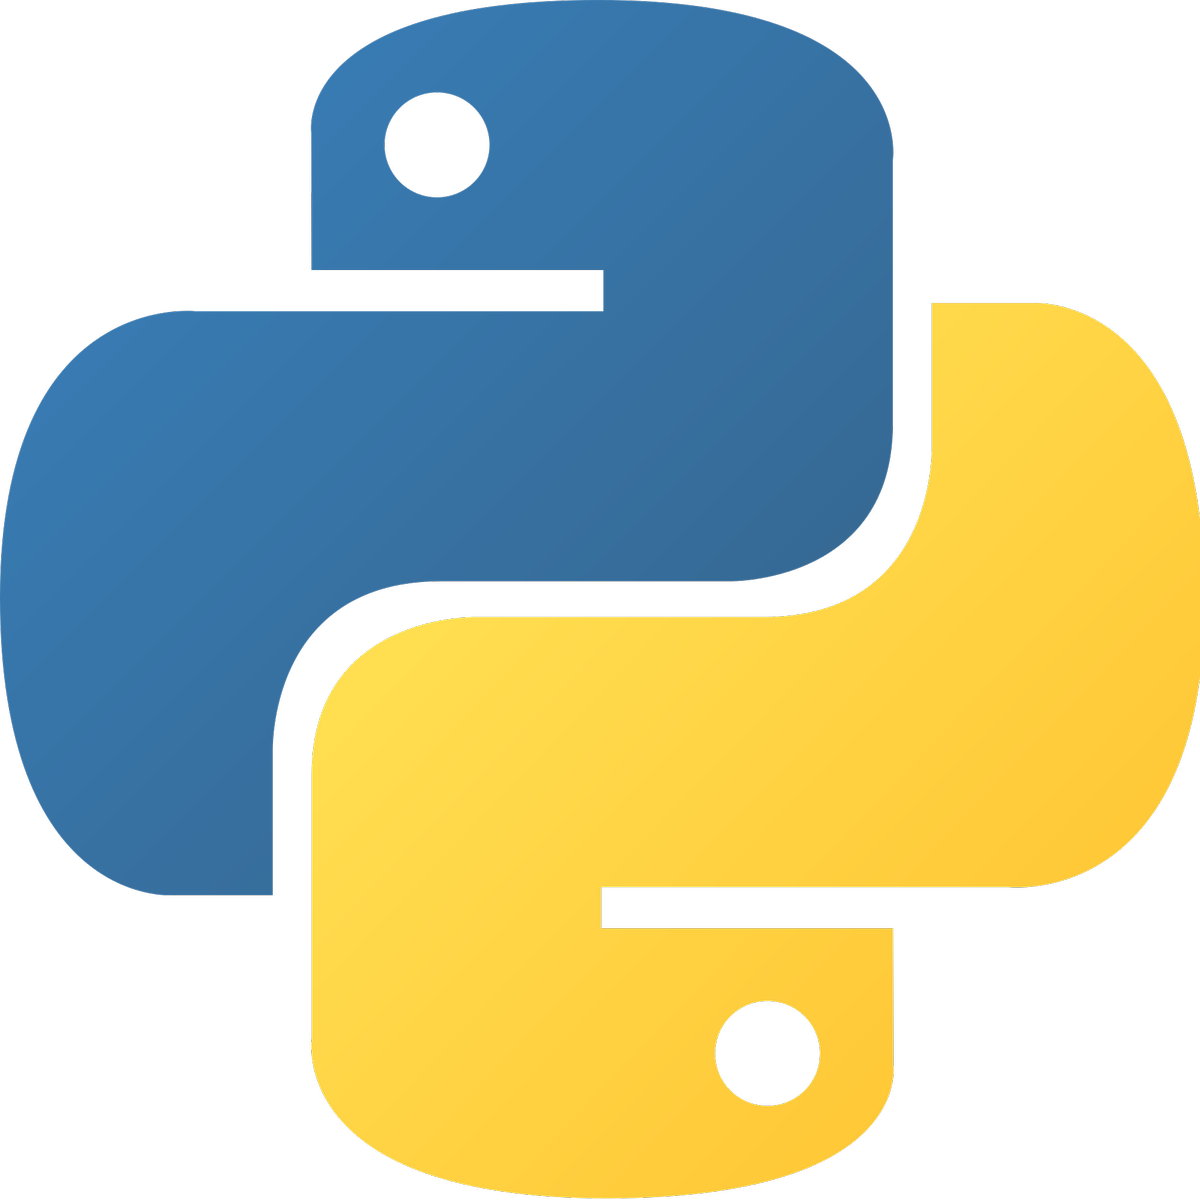
\includegraphics[width=3cm]{logo1} \quad
	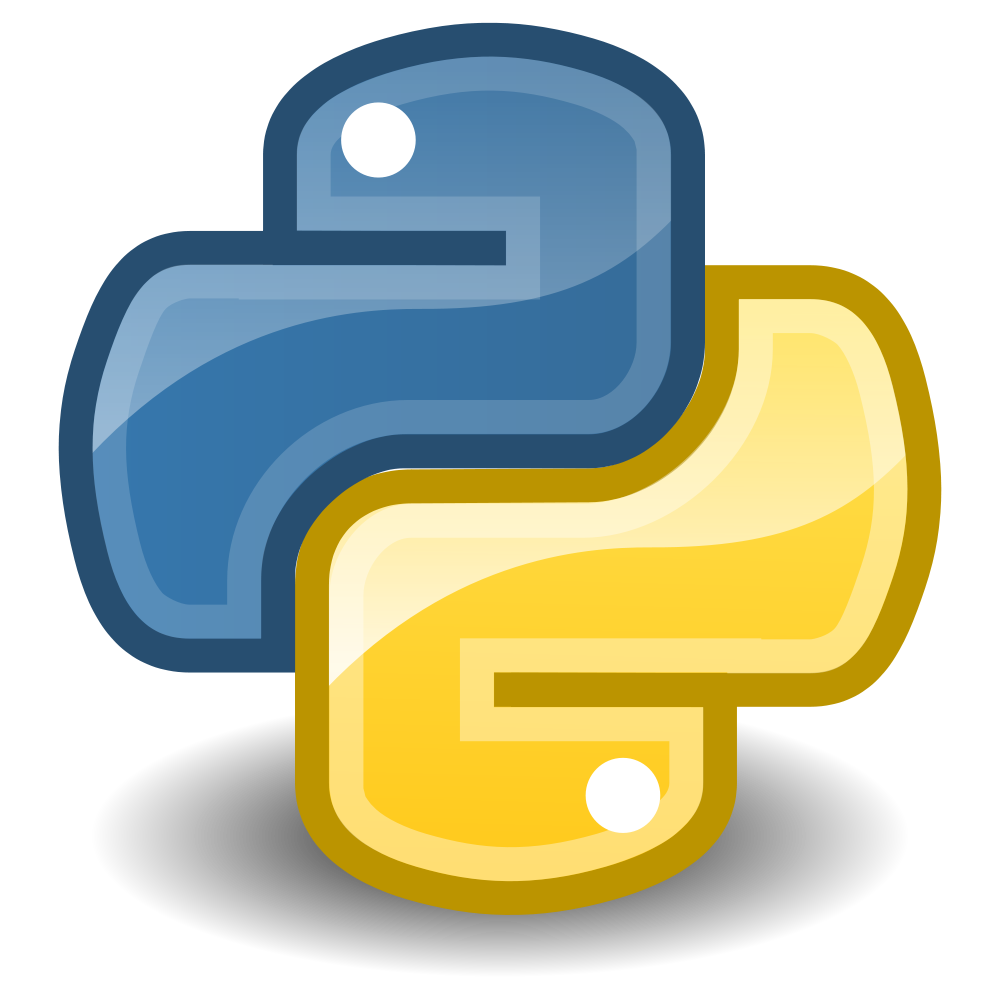
\includegraphics[width=3cm]{logo2} \quad
	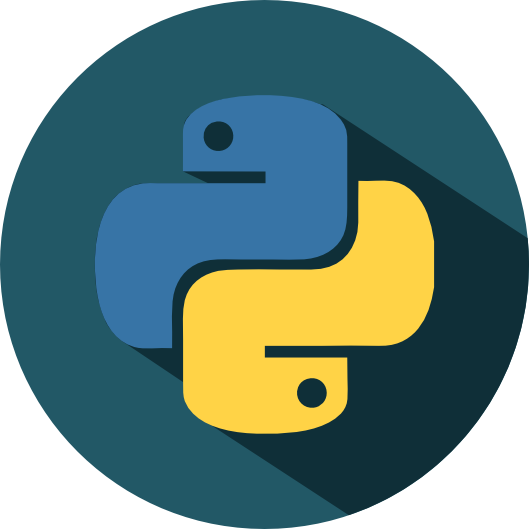
\includegraphics[width=3cm]{logo3} \newline
	Fonte: \url{www.pngwing.com}
\end{center}
\end{figure}


Dessa forma, conclui-se que o Python \'{e} uma linguagem de programa\c{c}\~{a}o vers\'{a}til e popular que \'{e} utilizada em diversas \'{a}reas, que v\~{a}o desde IA (Intelig\^{e}ncia Artificial) at\'{e} a an\'{a}lise de dados. Como possui uma sintaxe simplista e leg\'{\i}vel a linguagem torna-se f\'{a}cil de aprender e usar, fornecendo aos programadores uma s\'{e}rie de ferramentas e recursos proporcionada pela grande variedade de bibliotecas e estruturas. Como Python est\'{a} se tornando cada vez mais popular provavelmente prosseguir\'{a} a interpretar um papel relevante na \'{a}rea da tecnologia e do software.
  
%%%=========================================================================================%%%
   \section{\'{A}reas de Aplica\c{c}\~{a}o da Linguagem}
%%%=========================================================================================%%%
Python \'{e} uma linguagem de programa\c{c}\~{a}o muito vers\'{a}til que pode ser aplicada em diversas \'{a}reas da tecnologia como, por exemplo big data, orienta\c{c}\~{a}o a objetos, desenvolvimento web e an\'{a}lise de dados.

%%%.........................................................................................%%%
        \subsection{Big Data}
%%%.........................................................................................%%%
De acordo com \cite{McKinney2018}, a linguagem de programa\c{c}\~{a}o Python \'{e} altamente utilizada no campo da big data por possuir a capacidade de tratar uma larga escala de dados e de realizar o processamento paralelo. Al\'{e}m de dispor in\'{u}meras bibliotecas e frameworks para o tratamento de big data ela \'{e} uma linguagem de f\'{a}cil aprendizado.\newline

As principais \'{a}reas de big data em que s\~{a}o utilizados o Python:

\begin{itemize} [itemsep=5pt, parsep=5pt]
\item An\'{a}lise de dados: Python \'{e} utilizado para a an\'{a}lise de dados por dispor in\'{u}meras bibliotecas de an\'{a}lise de dados. As principais utilizadas nessa \'{a}rea s\~{a}o Pandas, NumPy, SciPy, Matplotlib, que possibilitam os desenvolvedores a realizar procedimentos como processamento de dados em larga escala, an\'{a}lise estat\'{\i}stica e visualiza\c{c}\~{a}o de dados.

\item Machine Learning (Aprendizado de M\'{a}quina): Tratando-se de uma das mais utilizadas linguagens de programa\c{c}\~{a}o para a elabora\c{c}\~{a}o de modelos de aprendizado de m\'{a}quina. Python possui TensorFlow, Scikit-learn e PyTorch como bibliotecas famosas de machine learning.

\item Processamento de dados em tempo real: Proporcionando aos programadores um processamento de larga escala de dados e uma resposta mais veloz a eventos em tempo real, as ferramentas como Apache Storm e Apache Kafka s\~{a}o para o processamento de dados em tempo real e amplamente utilizadas em Python.

\item Processamento de dados distribu\'{\i}dos: As ferramentas de sistemas de processamento de dados como Apache Spark e Apache Hadoop de Python possibilitam que programadores processem em larga escala conjuntos de dados em clusters distribu\'{\i}dos de computadores.\newline

\end{itemize} 

Desse modo, devido a possuir uma vasta diversidade de bibliotecas e frameworks, flexibilidade e tamb\'{e}m ser de f\'{a}cil uso, a linguagem de programa\c{c}\~{a}o Python \'{e} uma das principais escolhas para ser utilizada em big data, por existir uma demanda por big data em cont\'{\i}nuo crescimento, Python provavelmente prosseguir\'{a} se tornando uma escolha cada vez mais popular em big data.
        
%%%.........................................................................................%%%		
	\subsection{Orientação a objetos}
%%%.........................................................................................%%%
Entre um mar de linguagens de programa\c{c}\~{a}o orientadas a objetos (POO), o Python, que possui a orienta\c{c}\~{a}o a objetos como parte essencial da linguagem, se destaca fornecendo suporte completo para esse tipo de programa\c{c}\~{a}o. De acordo com \cite{Feltrin2019, Feltrin2020}, a programa\c{c}\~{a}o orientada a objetos \'{e} dedicada \`{a} cria\c{c}\~{a}o de objetos com atributos e m\'{e}todos, organizando-os em classes, hierarquia e heran\c{c}as, servindo assim como um meio de desenvolvimento de software. Al\'{e}m do mais, o Python permite que desenvolvedores criem c\'{o}digos mais modulares e vers\'{a}teis, atrav\'{e}s do polimorfismo em que as classes podem executar o mesmo m\'{e}todo de diferentes maneiras. Ainda, a linguagem de programa\c{c}\~{a}o Python possui uma biblioteca padr\~{a}o poderosa em POO chamada "pickle", que \'{e} utilizada para fazer a desserializa\c{c}\~{a}o e serializa\c{c}\~{a}o de objetos e outra chamada "abc" para definir interfaces e classes abstratas.

Alguns conceitos da orienta\c{c}\~{a}o a objetos em Python:

\begin{itemize} [itemsep=5pt, parsep=5pt]

\item Classes - A classe \'{e} usada para a cria\c{c}\~{a}o de objetos e definir seus m\'{e}todos e atributos.
\subitem Exemplo: A classe chamada 'Pessoa' recebe os atributos: 'nome' e 'idade'.

\item Heran\c{c}a - A heran\c{c}a em Python \'{e} utilizada para a cria\c{c}\~{a}o de novas classes com caracter\'{\i}sticas como atributos e m\'{e}todos, herdadas de classes que j\'{a} existem.
\subitem Exemplo: Uma nova classe 'Faculdade' herda os atributos da classe 'Aluno', podendo ser adicionados novos atributos nessa classe como, 'curso' e 'matr\'{\i}cula'.

\item Hierarquia - Na linguagem de programa\c{c}\~{a}o Python, \'{e} poss\'{\i}vel criar uma hierarquia de classes, ou seja, uma classe \'{e} a "principal" em rela\c{c}\~{a}o a outras classes.
\subitem Exemplo: A classe 'Cachorro' \'{e} a principal em rela\c{c}\~{a}o a classe como 'ra\c{c}a', a qual recebe atributos 'nome' da classe principal, al\'{e}m de ter seus pr\'{o}prios atributos 'cor' e 'porte'.

\item Polimorfismo - Com o polimorfismo \'{e} poss\'{\i}vel criar um m\'{e}todo em uma classe, podendo ser executado de diversas formas.
\subitem Exemplo: Temos a classe 'Pessoa' e outras classes que herdam dela: 'Aluno' e 'Professor', as duas possuem um m\'{e}todo chamado 'matricular' por\'{e}m cada uma implementa de uma forma diferente. \newline

\end{itemize}

Dessa forma, Python \'{e} uma linguagem boa que suporta programa\c{c}\~{a}o orientada a objetos, utilizada frequentemente em desenvolvimento de aplicativos web, desenvolvimentos de jogos, desenvolvimento de aplicativos desktop e etc. Escolhido principalmente por possuir um sintaxe simplista e de f\'{a}cil aprendizagem.
       
%%%.........................................................................................%%%
		\subsection{Desenvolvimento Web}
%%%.........................................................................................%%%
Python \'{e} uma linguagem de programa\c{c}\~{a}o amplamente utilizada no desenvolvimento web, especialmente devido a ter uma vasta diversidade de bibliotecas e frameworks. Os frameworks mais utilizados para o desenvolvimento web s\~{a}o Flask e Django, por\'{e}m existem outros frameworks em Python que s\~{a}o importantes para o desenvolvimento web, como o Pyramid.

De acordo com \cite{BarrosMaciel2020}, os Frameworks em Python utilizados em desenvolvimento web:

\begin{itemize} [itemsep=5pt, parsep=5pt]

\item Django - Um dos frameworks web mais utilizados em Python. Usando o Django criar sites ou aplicativos web escal\'{a}veis e seguros se torna muito f\'{a}cil, pois com ele \'{e} poss\'{\i}vel a cria\c{c}\~{a}o completa desses em pouco tempo, por possuir muitos recursos integrados, como o gerenciamento de URL, autentica\c{c}\~{a}o de usu\'{a}rios e a administra\c{c}\~{a}o de banco de dados.  

\item Flask - Um framework web de aprendizado mais f\'{a}cil que o Django. O Flask \'{e} usado para desenvolver aplica\c{c}\~{o}es web com incomplexidade e rapidez, possuindo como principal caracter\'{\i}stica a facilidade em criar rotas e funcionalidades web.

\item Pyramid - O framework web Pyramid para Python \'{e} o que possui maior flexibilidade e extensividade em rela\c{c}\~{a}o ao Django e ao Flask. Visto que, ele \'{e} apropriado para o desenvolvimento de grandes e complexos aplicativos web, por oferecer autentica\c{c}\~{a}o, cache, seguran\c{c}a e internacionaliza\c{c}\~{a}o que s\~{a}o uma grande diversidade de recursos.  \newline

\end{itemize}

Portanto, a linguagem de programa\c{c}\~{a}o Python \'{e} utilizado em diversas \'{a}reas do desenvolvimento web, que v\~{a}o desde a constru\c{c}\~{a}o de aplicativos web at\'{e} a an\'{a}lise de dados. Python oferece uma grande diversidade de bibliotecas e frameworks que atendem a todas as necessidades de desenvolvimento web, sem depender do tamanho e da dificuldade do projeto.

%%%.........................................................................................%%%        
		\subsection{An\'{a}lise de Dados }
%%%.........................................................................................%%%        
A linguagem Python possui uma diversidade de bibliotecas dispon\'{\i}veis e facilidade de uso tornando-a bem popular em an\'{a}lise de dados - que consiste em coletar, processar e analisar dados para adquirir informa\c{c}\~{o}es relevantes e insights sobre um determinado tema, sendo utilizada em diferentes \'{a}reas, como sa\'{u}de, marketing e finan\c{c}as. As bibliotecas Pandas, NumPy, Matplotlib e SciPy s\~{a}o as mais populares de Python que s\~{a}o empregues nessa \'{a}rea.

De acordo com \cite{McKinney2023, Chen2018}, a an\'{a}lise de dados em Python abrange um conjunto de etapas, a primeira etapa na an\'{a}lise de dados em Python \'{e} coletar os dados relevantes para o problema em quest\~{a}o. Ap\'{o}s realizar a coleta desses dados, \'{e} fundamental prepar\'{a}-los para uma an\'{a}lise. Nesta, \'{e} poss\'{\i}vel ser inclu\'{\i}do o preenchimento de dados ausentes, a limpeza de dados, regulariza\c{c}\~{a}o de dados e a transforma\c{c}\~{a}o desses em formatos apropriados para a an\'{a}lise. Logo ap\'{o}s \'{e} realizado uma an\'{a}lise explorat\'{o}ria de dados (EDA), que \'{e} uma t\'{e}cnica a qual possui como finalidade compreender o grupo de dados, examinando a sua distribui\c{c}\~{a}o, identificando os prov\'{a}veis padr\~{o}es, as tend\^{e}ncias e os v\'{\i}nculos entre as vari\'{a}veis. Al\'{e}m da EDA \'{e} realizada a an\'{a}lise estat\'{\i}stica que \'{e} um procedimento para conhecer as rela\c{c}\~{o}es entre vari\'{a}veis do conjunto de dados. Podendo ser inclu\'{\i}das a an\'{a}lise de correla\c{c}\~{o}es, regress\~{a}o e outras t\'{e}cnicas estat\'{\i}sticas. Ap\'{o}s essas an\'{a}lises, ocorre a modelagem preditiva, que abrange a cria\c{c}\~{a}o de modelos estat\'{\i}sticos para prever efeitos futuros com base nos dados \`{a} disposi\c{c}\~{a}o. A \'{u}ltima etapa da an\'{a}lise de dados em Python realiza a apresenta\c{c}\~{a}o das descobertas da an\'{a}lise de dados de maneira clara e sucinta.

Python em an\'{a}lise de dados realiza um processo iterativo envolvendo diversas etapas, que v\~{a}o desde a coleta de dados at\'{e} o relat\'{o}rio dos resultados. Alguns exemplos de \'{a}reas em que \'{e} largamente usada:

\begin{itemize} [itemsep=5pt, parsep=5pt, topsep=5pt]
  	 	
	\item Finan\c{c}as: Utilizada para realizar a an\'{a}lise de risco, previs\~{a}o de pre\c{c}os e gest\~{a}o de investimentos. 
	
	\item Sa\'{u}de: Usada para prever predisposi\c{c}\~{o}es de sa\'{u}de e reconhecer tratamentos mais eficazes.
	
\end{itemize}

Finda-se ent\~{a}o que a an\'{a}lise de dados em Python est\'{a} em um constante evolu\c{c}\~{a}o, tornando-se poderosa na extra\c{c}\~{a}o de informa\c{c}\~{o}es custosas de um amplo conjunto de dados. Possuindo ferramentas capazes de realizar tarefas desde um simples processamento de dados at\'{e} an\'{a}lises profundas de Machine Learning (Aprendizado de M\'{a}quina).